\documentclass[titlepage,11pt]{article}
\usepackage{tikz}
\usetikzlibrary{shapes.geometric, arrows}
\usepackage{multirow}
\usepackage{floatrow}
\usepackage{amsmath}
\begin{document}

\title{Software Systems Lab 4:\\TeX Lab}
\author{Team Contour}
\date{12 August, 2017}
\maketitle

\newpage

% Flowchart
\begin{figure} \label{flowchart}
\centering
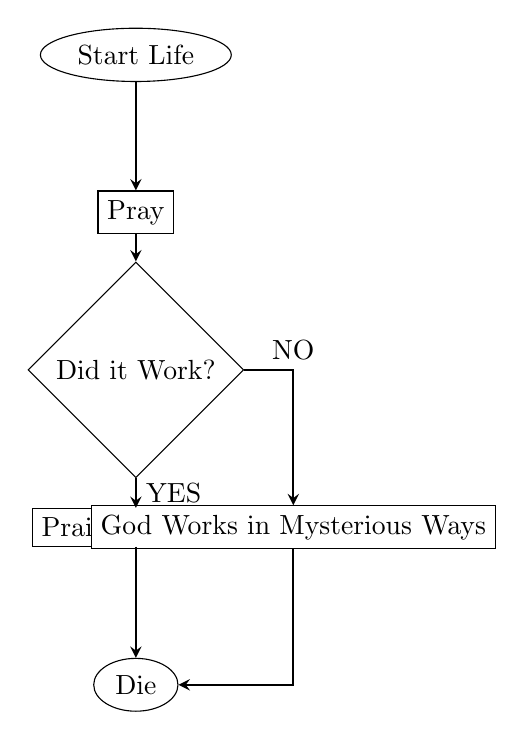
\begin{tikzpicture}[node distance=2cm]
\tikzstyle{oval}=[ellipse,text centered, draw=black, fill=white]
\tikzstyle{box}=[rectangle,text centered, draw=black, fill=white]
\tikzstyle{dia}=[diamond, text centered, draw=black, fill=white]
\tikzstyle{arrow}=[thick,->,>=stealth]
\node[oval] (st) {Start Life};
\node[box,below of=st] (b1) {Pray};
\node[dia, below of=b1] (if1) {Did it Work?};
\node[box, below of=if1] (b2) {Praise the Lord};
\node[box, right of=b2] (b3) {God Works in Mysterious Ways};
\node[oval, below of=b2] (end) {Die};
\draw[arrow] (st) -- (b1);
\draw[arrow] (b1) -- (if1);
\draw[arrow] (if1) -- node[anchor=west]{YES} (b2);
\draw[arrow] (if1) -| node[anchor=south]{NO} (b3);
\draw[arrow] (b3) |- (end);
\draw[arrow] (b2) -- (end);
\end{tikzpicture}
\caption{Flowchart of a theist life}
\end{figure}

% Paragraph
\paragraph{} Figure \ref{flowchart} above refers to a funny conundrum theists are believed to be living in by the atheists. This is just a joke I picked up from some forum, not taking sides, not even a bit. This is how scared social media has made us, We can not pick sides. Moving on\ .\ .\ .\ . You need to know how to cite papers in \LaTeX. For e.g. you are talking about research on Indowordnet \cite{indowordnet}, in that case such a citation must be used near a name. In case you need to quote the authors of a paper in a statement, instead of citing them against a topic or word or a line, you need to use a different kind of citation methodology.

% % Table
\begin{table}[h]
\centering
\caption{Table depicting the use of both multirow and multicolumn}
\begin{tabular}{c c|c|c|c|c|c|c|c|c|c|}
\cline{3-11}
& & \multicolumn{5}{c|}{\textbf{Basic Properties}} & \multicolumn{4}{c|}{\textbf{Readability}} \\ \cline{3-11}
& & \multicolumn{1}{|c|}{\textbf{WC}} & \textbf{SC} & \textbf{C-W} & \textbf{S-W} & \textbf{W-S} & \textbf{FK} & \textbf{GF} & \textbf{SMOG} & \textbf{LEX}\\ \cline{1-11}
\multicolumn{1}{|c|}{\multirow{2}{*}{\textit{Baseline}}} & Mean & 0.84 & 0.41 & \textbf{0.56} & \textbf{0.46} & \textbf{0.55} & \textbf{0.60} & 0.56 & 0.57 & 0.63\\ \cline{2-11}
\multicolumn{1}{|c|}{} & SD & 0.07 & 0.08 & 0.06 & 0.07 & 0.05 & 0.05 & 0.06 & 0.07 & 0.05\\ 
\hline \hline
 \multicolumn{1}{|c|}{\multirow{2}{*}{\textit{ScaComp$_{h}$}}} & Mean & 0.84 & 0.41 & \textbf{0.56} & \textbf{0.46} & \textbf{0.55} & \textbf{0.60} & 0.56 & 0.57 & 0.63\\ \cline{2-11}
\multicolumn{1}{|c|}{} & SD & 0.07 & 0.08 & 0.06 & 0.07 & 0.05 & 0.05 & 0.06 & 0.07 & 0.05\\ 
\hline \hline
\multicolumn{1}{|c|}{\multirow{2}{*}{\textit{ScaComp$_{l}$}}} & Mean & 0.84 & 0.41 & \textbf{0.56} & \textbf{0.46} & \textbf{0.55} & \textbf{0.60} & 0.56 & 0.57 & 0.63\\ \cline{2-11}
\multicolumn{1}{|c|}{} & SD & 0.07 & 0.08 & 0.06 & 0.07 & 0.05 & 0.05 & 0.06 & 0.07 & 0.05\\ 
\hline
\end{tabular}
\end{table}


% Conclusion
\section*{Conclusion} \label{end}
This document comprehensively demonstrated the capabilities of \LaTeX as a document typesetting / desktop publishing package. We have used various font size / family settings, we have used verbatim to display Latex code in a latex document, image settings, sections, subsections, references using labels, mathamatical equations, notations, use of ‘dia’ for creating a diagram / flowchart etc. I hope this suffices the need of learning basic \LaTeX. I hope you also notice that the last section i.e. Conclusion on Page \pageref{end} is unnumbered and displays the use of something.

% Bibliography
\begin{thebibliography}{9}
\bibitem{indowordnet}
Pushpak Bhattacharyya. Indowordnet. In \textit{The WordNet in Indian
Languages}, pages 1–18. Springer, 2017.
\end{thebibliography}

\end{document}